\chapter{Momentum and Angular Momentum}
\section{Conservation of Momentum}
Previously we stated the law of conservation of momentum, which states that for a system of $N$ particles, the rate of change of linear momentum on the system $\mbf{P} = \sum_\alpha \mbf{p}_\alpha$ is determined by the net external force on the system
\[ \mbf{\dot P} = \mbf{F}^{\text{ext}} \]
so if the net external force is zero, the total momentum is constant. This principle can help us solve many problems, such as the one below.
\begin{example}
    Two bodies have masses $m_1$ and $m_2$ and are travelling at velocities $\mbf{v}_1$ and $\mbf{v}_2$ before colliding with each other and sticking together, moving with some final velocity $\mbf{v}_\text{fin}$. Find $\mbf{v}_\text{fin}$. 

    The principle of conservation of momentum tells us that the total momentum on the system is the same before and after the collision, since there are no external forces. The momentum just before the collision is
    \[ \mbf{P}_{\text{in}} = m_1\mbf v_1 + m_2\mbf v_2 \]
    and the momentum just after is
    \[ \mbf{P}_{\text{fin}} = m_1\mbf v_\text{fin} + m_2\mbf v_\text{fin} = (m_1 + m_2)\mbf{v}_\text{fin}\]
    Equating these two, we have
    \[ (m_1+m_2)\mbf{v}_\text{fin} = m_1\mbf v_1 + m_2\mbf v_2 \]
    and then dividing by $m_1+m_2$,
    \[ \mbf{v}_\text{fin} = \frac{m_1\mbf v_1 + m_2\mbf v_2}{m_1+m_2}\]
\end{example}
\section{Rockets}
One large application of the principle of conservation of momentum is in the physics behind rockets. The basic question a rocket must answer is this: With no external agent to push you, how do you accelerate yourself? 

To answer this question, imagine you are trapped in the middle of a completely frictionless frozen lake. It is impossible to accelerate yourself by walking, as there is no friction to let you move. The simplest way to accelerate yourself is to throw something with a lot of mass in the opposite direction you want to go. As you throw the object, the reaction force from you throwing it pushes you backwards.

Rockets make use of this idea to its extreme. The rocket's motor hurls fuel into the air behind it, which pushes the rocket forward.

To analyze this situation mathematically, consider a rocket with mass $m$, traveling in the positive $\xhat$ direction and ejecting fuel with a velocity $v_\text{ex}$ relative to the rocket. At a time $t$, the rocket's momentum is $P(t) = mv$. At time $t + \dd t$, the mass of the rocket is $m + \dd m$, where $\dd m$ is negative, and its momentum is $(m + \dd m)(v + \dd v)$. The fuel ejected in that time $\dd t$ has mass $-\dd m$ and a velocity of $v - v_\text{ex}$ relative to the ground. 

Thus the total momentum of the rocket-fuel system at $t+\dd t$ is
\begin{align*}
    P(t + \dd t) &= (m+\dd m)(v+\dd v) - \dd m(v - v_\text{ex}) \\
    &= mv + v\dd m + m \dd v + \dd m \dd v - v\dd m + v_\text{ex}\dd m  \\
    &\approx mv + m \dd v + v_\text{ex}\dd m 
\end{align*}
where the $\dd m \dd v$ term is disregarded because of its tiny size, as the product of two differentials. 

The change in momentum is $\dd P = P(t + \dd t) - P(t) = m\dd v + v_\text{ex}\dd m$. If there is some external force $F^\text{ext}$ (gravity, for instance), then $\dd P = F^\text{ext}$. Here, we will assume there is no external force, so $\dd P = 0$. This allows us to write
\[ m \dd v = -v_\text{ex}\dd m \]
or
\begin{equation} \label{thrust}
     m \dot v = -v_\text{ex}\dot m 
\end{equation}
Where $\dot m$ is the rate at which the rocket's engine is ejecting mass. This equation is essentially the equivalent of Newton's Second Law for rockets, where $-v_\text{ex}\dot m$ plays the role of the force. For this reason, we refer to the quantity $-v_\text{ex}\dot m$ as the \textbf{thrust} of the rocket. 

Because $\dot m$ is negative, the thrust is a positive quantity. 

(\ref{thrust}) is a separable differential equation and can be solved quite easily:
\begin{align*}
    \int_{v_0}^v\dd v &= -v_\text{ex} \int_{m_0}^m \frac{\dd m}{m} \\
    v - v_0 &= v_\text{ex}\ln(m_0/m)
\end{align*}
This result puts a significant restriction on the speed of the rocket. The increase in speed is determined by the size of the term $\ln(m_0/m)$, which is at its maximum when all fuel is burned and the remaining mass is just the rocket itself and the payload. 

Even if $90\%$ of the rocket's mass is fuel that was burned, $\ln(m_0/m)$ is still only equal to about $2.3$, and the velocity cannot be more than $2.3$ times bigger than $v_\text{ex}$. To combat this, rocket engineers spend a significant amount of time trying to maximize $v_\text{ex}$ and reduce the final mass (this is why rockets often detach from their fuel tanks after emptying them). 

\section{Center of Mass}
Consider a group of $N$ particles with masses $m_i$ and positions $\mbf{r}_i$ measured relative to some origin $O$. The \textbf{center of mass} of this system is defined as the position relative to $O$ given by
\[ \mbf R = \frac{\sum m_i\mbf{r}_i}{\sum m_i}\]
by writing the total mass of the system as $M = \sum m_i$, then $\mbf R = \frac{1}{M}\sum m_i\mbf{r}_i$. This equation can be quite easily split into three equations, one for each component.

Another way to think about the center of mass $\mbf{R}$ is as a weighted average of all the individual positions, with each $\mbf{r}_i$ having a weight of $m_i$. 

In the case where there are only two masses, the center of mass is
\[ \mbf{R} = \frac{m_1\mbf{r}_1 + m_2\mbf{r}_2}{m_1+m_2} \]
From this definition, it is pretty simple to show that the center of mass of $m_1$ and $m_2$ lies on the line joining $\mbf{r}_1$ and $\mbf{r}_2$, and the ratio of the distances between ($\mbf{R}$ and $\mbf{r_1}$) and ($\mbf{R}$ and $\mbf{r}_2$) is equal to $m_1/m_2$. 

If $m_1$ is much greater than $m_2$, then $\mbf{R} \approx \mbf{r}_1$, and vice versa if $m_2$ is much greater than $m_1$. This also extends to the $N$-particle case--if $m_1$ is much greater than all of the other masses, then $\mbf{R}\approx \mbf{r}_1$. An example of this is our solar system. The sun is much more massive than every other planet (and all of the non-planet objects as well), so the center of mass of the solar system is approximately equal to the position of the sun. 

We are also able to write
\[ M\mbf{R} = \sum m_i\mbf{r}_i\]
And then differentiate to find
\[ M\mbf{\dot R} = \sum m_i \mbf{\dot r}_i \]
But $\sum m_i\mbf{\dot r}_i$ is just the total momentum of the system. Therefore,
\[ \mbf{P} = M\mbf{\dot R} \]
We can differentiate once again and use $\mbf{F}^\text{ext} = \mbf{\dot P}$ to write
\[ \mbf{F}^\text{ext} = M\mbf{\ddot R}\]
This shows an extremely crucial result that allows us to generalize many of our results from studying particles to actual scenarios--the center of mass of a system of particles moves exactly as if it were a single particle of mass $M$.

The concept of the center of mass can be extended to continuous distributions of mass using integration. For some three-dimensional volume $V$ with a mass distribution $\rho(x,y,z)$, then
\[ \mbf{R} = \frac{1}{M} \iiint\limits_V \rho \, \mbf{r}\, \dd V \]
where $M = \iiint\limits_V \rho \, \dd V$ is the mass of $V$. The same concepts apply to one-dimensional or two-dimensional mass distributions.
\begin{example}[Center of Mass of a Solid Cone]
    A cone with a constant density $\rho$ has a radius of $R$ and a height $h$. Find its center of mass. 

    It makes the most sense to analyze this problem through cylindrical coordinates. We will orient our cone so that its vertex is at the origin $O$, and it gets wider as the $z$ coordinate increases. At each height $z$, the horizontal cross section is a circle of radius $r = Rz/h$. We can rearrange this to $z = hr/R$, and set up our triple integral as 
    \begin{align*}
        \mbf R = \frac{1}{M} \iiint\limits_V \rho \mbf r \dd V &= \frac{1}{M} \int_0^{2\pi}\int_0^{R}\int_{hr/R}^h \rho r \mbf r \dd z \dd r \dd \theta
    \end{align*}
    But before we evaluate this, we should first find the mass $m$.
    \begin{align*}
        M = \iiint\limits_V \rho \dd V &= \int_0^{2\pi}\int_0^R\int_{hr/R}^h \rho r\dd z\dd r\dd \theta \\
        &= 2\pi\rho \int_0^R \pqty{rh - \frac{r^2h}{R}}\dd r \\
        &= 2\pi\rho \pqty{\frac{R^2h}{2} - \frac{R^2h}{3}} = \frac{1}{3}\rho \pi R2 h 
    \end{align*} 
    We then divide the vector $\mbf{r}$ into its components and handle them separately. First, the $x$ component:
    \begin{align*}
        R_x &= \frac{1}{M} \int_0^{2\pi}\int_0^{R}\int_{hr/R}^h \rho r^2\cos\theta \dd z \dd r \dd \theta = 0  
    \end{align*}
    This is immediately zero because $\int_0^{2\pi}\cos\theta\, \dd\theta = 0$. By similar logic, the $y$ component goes to zero as well:
    \[ R_y = \frac{1}{M} \int_0^{2\pi}\int_0^{R}\int_{hr/R}^h \rho r^2\sin\theta \dd z \dd r \dd \theta = 0  \]
    It makes sense for both of these integrals to be zero because of the circular symmetry of the cylinder about the $z$ axis. Finally, we will compute the $z$ component.
    \begin{align*}
        R_z &= \frac{1}{M} \int_0^{2\pi}\int_0^{R}\int_{hr/R}^h \rho rz \dd z \dd r \dd \theta \\
        &= \frac{\pi\rho h^2}{M} \int_0^R \pqty{r - \frac{r^3}{R^2}} \dd r \\
        &= \frac{\pi \rho h^2}{2M} \pqty{R^2 - \frac{R^2}{2}} \\
        &= \frac{\pi \rho h^2R^2}{4M} = \frac{3}{4}h
    \end{align*}
    So the cartesian coordinates of the center of mass of the cone are $(0, 0, 3h/4)$.
\end{example}
\section{Angular Momentum for a Single Particle}
We define the \textbf{angular momentum} of a single particle as the vector
\[ \bm{\ell} = \mbf{r} \times \mbf p\]
Notice that because $\bm\ell$ depends on the position vector $\mbf{r}$, it will vary depending on our choice of origin. For this reason, we will often say that $\bm\ell$ is the angular momentum of the particle \textit{relative} to $O$.

We can also differentiate $\ell$ to find
\[ \bm{\dot \ell} = \dv{t} (\mbf{r}\times\mbf{p}) = \mbf{\dot r}\times \mbf{p} + \mbf{r}\times\mbf{\dot p} \]
Because $\mbf{p} = m\mbf{\dot r}$, the left cross product is simply zero and we get
\[ \bm{\dot \ell} = \mbf{r}\times\mbf{\dot p} = \mbf{r}\times\mbf{F} \]
We define this quantity as the net \textbf{torque} of the particle about $O$, and denote it with $\bm{\Gamma}$ (other texts may use $\bm{\tau}$ or $\mbf{N}$). 

We often think of
\begin{equation} \label{rotn2l}
    \bm{\Gamma} = \bm{\dot \ell}
\end{equation}
As the equivalent to Newton's Second Law for rotation. Indeed, it is common to think of $\bm{\Gamma}$ as the rotational equivalent to force. 

Oftentimes, we can choose the origin of our coordinate system such that the new torque is zero. For instance, consider a planet of mass $m$ orbiting around the sun (mass $M$). If we define the origin as the location of the sun, the net force on the planet is just the gravitational force, or
\[ \mbf{F} = -\frac{GmM}{r^2}\rhat \]
Then, by (\ref{rotn2l}),
\[ \bm{\Gamma} = \mbf{r} \times \mbf{F} = -\frac{GmM}{r^2} (\mbf{r}\times\rhat) = \mbf{0}\]
Forces with the property that $\mbf F = k\rhat$ for some constant $k$ are called \textbf{central forces}, and have a few special properties that prove useful. For one, as we have just shown, a central force exerts no torque on an object and thus preserves conservation of angular momentum. 
\subsection*{Kepler's Second Law}
One of the biggest triumphs of Newton's formulation for mechanics was that he was able to explain Kepler's second law with the principle of conservation of angular momentum. Kepler's laws were published eighty years before Newton's laws of motion, and were simply descriptions of the qualitative observations made by Kepler. They made no attempt to explain these observations in terms of fundamental ideas, but all of them turn out to be direct consequences of Newton's laws. We will speak about Kepler's first and third laws later, but for now we will focus on the second law.
\begin{theorem}[Kepler's Second Law]
    As each planet moves around the sun, a line drawn from the planet to the sun sweeps out equal areas in equal times. 
\end{theorem}
\begin{figure}[h!]
    \centering
    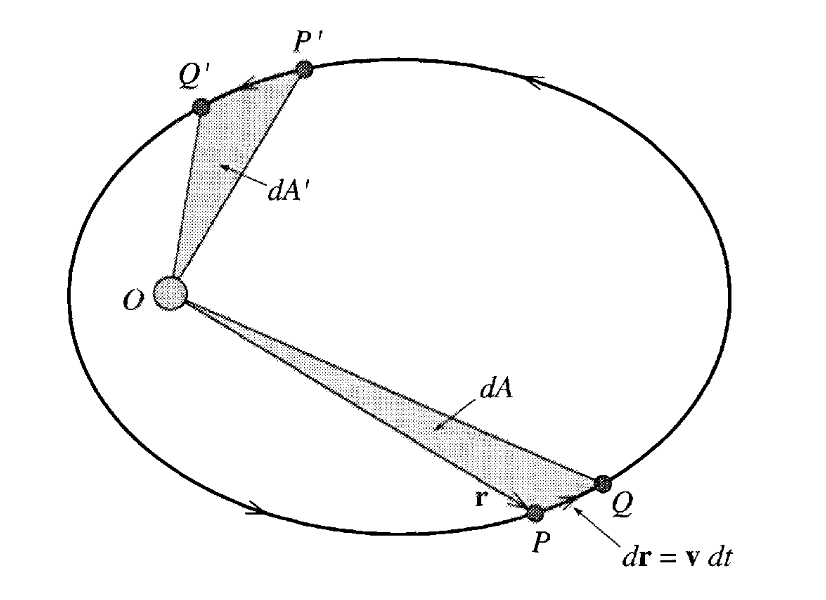
\includegraphics[width=0.5\linewidth]{keplerSecondLaw.png}
    \caption{Kepler's Second Law states that if the two pairs of points $P$, $Q$, $P'$, $Q'$ are separated by equal time intervals $\dd t = \dd t'$, then the two areas $\dd A$ and $\dd A'$ are equal.}
    \label{fig:keplerSecondLaw}
\end{figure}

To show this, we will approximate the area formed by the oval sector $OPQ$ as a triangle with vertices at $O$, $P$, and $Q$. Two of the sides of this triangle can be represented by the vectors $\mbf r$ and $\mbf \dd \mbf r$. Then, recall that the area of the triangle formed by $\mbf r$ and $\dd \mbf r$ is given by
\[ \dd A = \frac{1}{2}\abs{\mbf r \times \dd \mbf r} \]
But since $\dd \mbf r = \mbf v \dd t$, 
\[ \dd A = \frac{1}{2}\abs{\mbf r \times \mbf v \dd t} \]
then, diving by $\dd t$ and replacing $\mbf v$ with $\mbf p/m$,
\[ \frac{\dd A}{\dd t} = \frac{1}{2m}\abs{\mbf r \times \mbf p} = \frac{\ell}{2m} \]
Then, due to the conservation of angular momentum, $\dd A/\dd t$ is constant. This means that Kepler's Second Law is equivalent to the conservation of angular momentum. 

Notice that the proof of Kepler's Second Law depended only on the fact that the gravitational force is central and hence the angular momentum of the planet about $O$ is constant. This means that we can extend these results to any system where an object moves under the influence of just a central force. 
\section{Angular Momentum for Several Particles}
Consider a system of $N$ particles each with angular momentum $\bm{\ell}_i = \mbf{r}_i \times \mbf{p}_i$ relative to some origin $O$. We define the total angular momentum of the system as
\[ \mbf{L} = \sum_i \bm{\ell}_i = \sum_i \mbf{r}_i \times \mbf{p}_i \]
by differentiating with respect to $t$, we find
\begin{equation} \label{ldot1}
    \mbf{\dot L} = \sum_i \bm{\dot \ell}_i = \sum_i \mbf{r}_i \times \mbf{F}_i
\end{equation}
Every object in the system exerts a force on every other object in the system. Therefore, the net force on every particle can be represented as a sum of each internal force, plus the net force on the particle. 
\[ \mbf{F}_i = \sum _{i\neq j} \mbf{F}_{ij} + \mbf{F}^\text{ext}_i \]
Substituting this into (\ref{ldot1}), we find
\[ \mbf{\dot L} = \sum_{i}\sum_{i\neq j} (\mbf{r}_i \times \mbf{F}_{ij}) + \sum_i(\mbf{r}_i \times \mbf{F}^\text{ext}_i) \]
similar to how we worked with linear momentum, we regroup the left sum so it becomes
\begin{align*}
    \mbf{\dot L} &= \sum_i \sum_{j > i}(\mbf{r}_i \times \mbf F_{ij} + \mbf{r}_j \times \mbf F_{ji}) + \sum_i \mbf r_i\times \mbf{F}^\text{ext}_i \\
    &= \sum_i \sum_{j > i}((\mbf{r}_i - \mbf{r}_j)\times \mbf{F}_{ij}) + \sum_i \mbf r_i\times \mbf{F}^\text{ext}_i
\end{align*}
To show that $(\mbf{r}_i \times \mbf{r}_j)\times\mbf{F}_{ij}$, recall that $\mbf{r}_i - \mbf{r}_j$ gives the vector pointing from $\mbf{r}_i$ to $\mbf{r}_j$. Similarly, each force $\mbf{F}_{ij}$ points directly along the line connecting $\mbf{r}_i$ and $\mbf{r}_j$. This means that $\mbf{r}_i - \mbf{r}_j$ is parallel to $\mbf{F}_{ij}$, so their cross product is zero. This allows us to cancel the entirety of the first sum, so we are just left with
\[ \mbf{\dot L} = \sum_i \mbf{r}_i \times \mbf{F}^\text{ext}_i = \sum_i \bm{\Gamma}_i^\text{ext} = \bm{\Gamma}^\text{ext} \]
Therefore, as long as the net external torque of the system is zero, conservation of angular momentum holds for the $N$-particle case.
\begin{theorem}[Principle of Conservation of Angular Momentum]
    If the net external torque on an $N$-particle system is zero, the system's total angular momentum $\mbf L = \sum \mbf{r}_i \times \mbf{p}_i$ is constant.

    In particular, we have $\mbf{\dot L} = \bm{\Gamma}^\text{ext}$.
\end{theorem}
\subsection*{The Moment of Inertia}
The definition of the angular momentum $\mbf{L} = \sum \mbf{r}_i \times \mbf{p}_i$ of a system is certainly valid, but it involves a summation over every particle within the system, which often proves difficult to calculate, especially for rigid bodies which are made up of infinitely many particles of differential mass. To simplify calculations, the notion of a \bf{moment of inertia} was created.

If we take the axis of rotation of the object to be the $z$ axis, then the $z$ component of the angular momentum is given by $L_z = I_z\omega$ where $I_z$ is the moment of inertia of the system about the $z$ axis and $\omega$ is the angular velocity of rotation about the $z$ axis. In general, the moment of inertia about the $z$ axis for a multi-particle system is given by 
\[ I_z = \sum_i m_i r_{iz}^2 \]
where $r_{iz}$ is the distance of the mass $m_i$ from the axis of rotation. 
\subsection*{Angular Momentum about the Center of Mass}
The result $\mbf{\dot L}=\bm{\Gamma}^\text{ext}$ was derived based on the assumption that $\mbf L$ and $\bm{\Gamma}^\text{ext}$ are measured relative to some fixed origin $O$ in an \textit{inertial} reference frame $\mathcal{S}$. Remarkably, the same result holds if $\mbf{L}$ and $\bm{\Gamma}^\text{ext}$ are measured relative to the center of mass of a system--even if the center of mass is being accelerated.

We will prove this result when we look at the mechanics of inertial systems more in depth, but we mention it now as it is a useful result.
\begin{example}[A Sliding and Spinning Dumbbell]
    A dumbbell consisting of two equal masses $m$ mounted on the ends of a rigid massless rod of length $2b$ is at rest on a frictionless horizontal table, lying on the $x$ axis and centered on the origin. At time $t=0$, the left mass is given a sharp tap of force $\mbf{F}$ in the $y$ direction for a short time $\Delta t$. Describe the subsequent motion.

    This problem consists of two parts--the initial motion immediately after the impulse, and the continued motion after the end of the impulse. For the first section, the only force on the object is the applied force from the tap. The linear momentum is initially zero, and because $\mbf{\dot P} = \mbf{F}$, we can integrate to find that at $t=\Delta t$,
    \[ \mbf{P}(\Delta t) = \int_0^{\Delta t} \mbf{F}\dd t = \mbf{F}\Delta t \]
    Furthermore, since $\mbf{P} = M\mbf{\dot R}$, where $M=2m$ is the total mass of the system and $\mbf{R}$ is the position of the position of the center of mass of the system, we can conclude that the center of mass begins to move up the $y$ axis with velocity
    \[ \mbf{\dot R} = \frac{\Delta t}{2m}\mbf{F}\]
    The vector pointing from $\mbf{R}$ to the point of application of the tap is given by $\mbf r = -b\xhat - \mbf{R}$. If we choose the origin to be at the center of mass $\mbf{R}$ and assume that $\Delta t$ is small enough such that $\mbf{R}(t) \approx \mbf{R}(0)$ for $t < \Delta t$, then
    \[ \mbf r \approx -b\xhat \]
    and the torque applied by $\mbf{F}$ relative to the center of mass is approximately constant at
    \[ \mbf{\Gamma} \approx (-b\xhat) \times \mbf{F} = -Fb\zhat \]
    So the angular momentum in the $-\zhat$ direction at $t=\Delta t$ is approximately $L = Fb\Delta t$. This causes a counterclockwise rotation relative to the center of mass. We can then write $L = I\omega$, where $I = \sum m_i r_i^2 = 2mb^2$. This gives
    \[ Fb\Delta t \approx 2mb^2\omega\]
    or $\omega = F\Delta t/2mb$. This means that the left side of the dumbbell is moving with initial velocity
    \[ \mbf{v}_\text{left} = \mbf{\dot R} + \omega b\yhat = \frac{F\Delta t}{m}\yhat  \]
    relative to an outside observer and the right side of the dumbbell is moving with initial velocity
    \[ \mbf{v}_\text{right} = \mbf{\dot R} - \omega b\yhat = \mbf{0} \]
    relative to an outside observer. Thus only the left side of the dumbbell is moving; the right side is initially stationary.

    The subsequent motion is quite straightforward. Once the impulse has ceased, there are no external forces or torques. Thus the center of mass continues to move straight up the $y$ axis with constant speed and the dumbbell continues to rotate with constant angular velocity about the center of mass.
\end{example}